\documentclass[10pt,a4paper,twocolumn]{article}
\usepackage[margin=1.7cm]{geometry}
\usepackage{fontspec}
\setmainfont{TeX Gyre Termes}
\usepackage{graphicx,booktabs,amsmath,xcolor,hyperref,caption,enumitem}
\hypersetup{colorlinks,linkcolor=black,urlcolor=blue!50!black,citecolor=black}
\captionsetup{font=small,labelfont=bf}
\setlist{nosep,leftmargin=*}
\newcommand{\fig}[2]{\begin{figure}[!htb]\centering\includegraphics[width=\columnwidth]{../docs/figures/#1}\caption{#2}\end{figure}}
\title{\vspace{-1.2cm}\textbf{Path Finder: inertial-only 6-DoF trajectory estimation\\under progressive sensor degradation}}
\author{Raktim Chandra, Nipun Dewangan, Pronov Mazumdar\\ \small \texttt{\{rc8823, nd9844, pm2235\}@srmist.edu.in}\\ \small Team SRMIST\_vortexxx, SRM Institute of Science and Technology\\ \small Samsung PRISM XR Hackathon 2026, Track 03 \quad \url{https://github.com/RaktimChandra/pathfinder}}
\date{}
\renewcommand{\topfraction}{0.9}\renewcommand{\bottomfraction}{0.8}\renewcommand{\textfraction}{0.07}\renewcommand{\floatpagefraction}{0.85}\setcounter{totalnumber}{5}\setcounter{topnumber}{4}
\begin{document}
\maketitle
\begin{abstract}
We estimate a full 6-DoF trajectory from a single IMU whose quality degrades over time and which fails completely five seconds before the end, with no camera, GPS or waypoints. Textbook strapdown integration of the same inputs ends hundreds of metres to tens of kilometres off. Path Finder treats position as a smoothing problem: a 14-state linear-time-varying Kalman filter with an RTS smoother, fed by observations the IMU already contains. These are rotor-drag body velocity, rest periods, a bounded workspace and a noise model that follows the published degradation schedule. On 17 public sequences (EuRoC MAV, TUM-VI), each degraded with the organisers' script under two column readings, it beats a constant-position reference on all 34 files and on 36 further stress files. Mean ATE is 1.39\,m in the Vicon rooms, 3.95\,m in the 20\,m Machine Hall and 0.54\,m in the TUM-VI rooms. It runs in one NumPy file at 1.2--2.7\,ms per second of data with a 3.0\,MB peak heap.
\end{abstract}

\section{Problem}
The input is an EuRoC-format IMU stream (gyro and accelerometer, about 200\,Hz). The official \texttt{degrade\_imu.py} ramps its severity as $0.02+0.98(t/T)^{1.7}$ and adds white noise, bias random walk, scale drift, spikes, stuck samples, single and burst dropouts, and duplicated rows. It zeroes the last 5\,s, during which the vehicle keeps moving. The output is one TUM-format pose per input row. Scoring uses evo ATE after an SE(3) Umeyama alignment.

\section{Five measured facts}
\textbf{(1) Integration cannot find position.} Over 90\% of EuRoC position energy lies below 0.05\,Hz. With the true attitude and the true accelerometer bias supplied, naive integration still ends 27\,m off on clean V1\_01. Position therefore has to come from constraints, not integration.

\textbf{(2) A multirotor's accelerometer measures velocity.} Rotor drag makes the specific force perpendicular to the thrust axis proportional to body velocity, $f_\perp\approx k\,v_b$. We fit $k=[-0.166,-0.201]$\,s$^{-1}$ on the Vicon rooms with leave-one-out folds stable to $\pm0.01$. Fitted independently on the Machine Hall, $k=[-0.166,-0.215]$, so the model describes the vehicle and not the room.

\textbf{(3) Vehicles rest.} The rest before take-off gives the full gyro bias, including the vertical axis that gravity cannot observe, and zero-velocity updates. Later rest periods ($\geq$1.5\,s) give zero-velocity updates too.

\textbf{(4) Do not trust the last velocity.} Degradation peaks just before the failure, so the velocity estimate there is the least reliable of the whole flight. Holding position (velocity decay $\tau=0.2$\,s) beats extrapolating it (Fig.~\ref{fig:blind}).

\textbf{(5) Degradation has a schedule.} Process noise follows the official ramp and the measured excess gyro scatter, so late samples automatically count less. This is the single most important component (Table~\ref{tab:abl}).

\fig{architecture.png}{Pipeline. Everything runs in one file, single thread, NumPy only.}

\section{Estimator}
\textbf{Ingest and triage.} The column order is taken from the header and checked against physics (the accelerometer has a steady magnitude near $g$). Units and timestamp formats are detected automatically. Dead rows, stuck samples, spikes (running median plus MAD gate), duplicates and dropouts are handled. The platform is identified from the gravity direction in the sensor frame.

\textbf{Attitude.} A complementary filter. Gyro increments use a trapezoidal rate, so a dropout during fast rotation integrates correctly. They are composed within 0.1\,s blocks by a segmented parallel prefix product of quaternions, with gravity feedback once per block. Known multirotors use a body-frame gravity reference; anything else uses a world-frame reference averaged over seconds, which tolerates aggressive handheld motion.

\textbf{Translation.} A Kalman filter plus RTS smoother at 2.5\,Hz with state $[p,v,b_w,c,d]$: position, velocity, world acceleration offset, workspace centre and drag offset. Observations are block-mean world acceleration, rotor-drag velocity, zero velocity at rest, and a soft prior $\|p-c\|\sim\mathcal N(0,\sigma^2)$. The drag observation is Cauchy-weighted: when the normalised innovation squared exceeds 4, its noise is inflated in proportion, so it switches itself off when the vehicle is carried or parked. Output positions use cubic Hermite interpolation and orientations use nlerp, at every input row.

\section{Evaluation}
Inputs come from the official script, seed 42, under two readings: H1 (accelerometer noise on the accelerometer) and H2 (the EuRoC file fed as is). Ground truth covers the failure window. EuRoC drag constants are always leave-one-sequence-out. References: textbook strapdown and a constant position, both scored by the same evo pipeline.

\begin{table}[!htb]\centering\small
\caption{ATE RMSE [m], mean of H1 and H2. $\dagger$: first blind tests; $\ddagger$: Machine Hall (blind run failed, then fixed, Sec.~\ref{sec:mh}); $\S$: final blind tests on the frozen estimator.}
\begin{tabular}{lrrr}\toprule
Sequence & Strapdown & Constant & \textbf{Ours}\\\midrule
V1\_01 & 1.4\,km & 1.85 & \textbf{1.36}\\
V1\_02$^\dagger$ & 349\,m & 1.78 & \textbf{0.81}\\
V1\_03$^\dagger$ & 530\,m & 1.58 & \textbf{1.43}\\
V2\_01 & 830\,m & 2.30 & \textbf{2.03}\\
V2\_02 & 507\,m & 2.11 & \textbf{1.40}\\
V2\_03$^\S$ & 389\,m & 2.06 & \textbf{1.31}\\
MH\_01$^\ddagger$ & 50.4\,km & 4.33 & \textbf{3.88}\\
MH\_02$^\ddagger$ & 34.4\,km & 4.66 & \textbf{4.28}\\
MH\_03$^\ddagger$ & 31.5\,km & 3.58 & \textbf{2.31}\\
MH\_04$^\ddagger$ & 17.8\,km & 6.80 & \textbf{4.50}\\
MH\_05$^\ddagger$ & 1.6\,km & 6.87 & \textbf{4.78}\\
TUM room1 & 12.5\,km & 1.00 & \textbf{0.44}\\
TUM room2$^\dagger$ & 12.1\,km & 1.22 & \textbf{0.50}\\
TUM room3$^\dagger$ & 17.3\,km & 1.25 & \textbf{0.48}\\
TUM room4$^\S$ & 5.8\,km & 1.08 & \textbf{0.69}\\
TUM room5$^\S$ & 18.2\,km & 0.93 & \textbf{0.57}\\
TUM room6$^\S$ & 19.0\,km & 0.99 & \textbf{0.54}\\\bottomrule
\end{tabular}\label{tab:main}\end{table}

\begin{table}[!htb]\centering\small
\caption{Tier views, mean (ours / constant) [m].}
\begin{tabular}{lccc}\toprule
& Vicon & Hall & TUM-VI\\\midrule
ATE & \textbf{1.39}/1.95 & \textbf{3.95}/5.25 & \textbf{0.54}/1.08\\
Waypoints, 10\,s & \textbf{1.36}/1.93 & \textbf{4.05}/5.45 & \textbf{0.52}/1.12\\
Blind 5\,s & \textbf{2.00}/2.03 & \textbf{2.29}/4.21 & 0.73/\textbf{0.64}\\
After dropouts & \textbf{1.41}/1.93 & \textbf{3.10}/5.03 & \textbf{0.57}/1.02\\\bottomrule
\end{tabular}\label{tab:tier}\end{table}

\begin{table}[!htb]\centering\small
\caption{Ablation: mean ATE / blind-window RMSE [m].}
\begin{tabular}{lccc}\toprule
& Vicon & Hall & TUM-VI\\\midrule
\textbf{final} & \textbf{1.39}/2.00 & \textbf{3.95}/2.29 & \textbf{0.54}/0.73\\
$-$ rotor drag & 1.65/2.04 & 5.13/4.18 & 0.54/0.73\\
$-$ degradation noise & 2.51/4.96 & 5.81/8.86 & 1.25/2.69\\
$-$ robust drag & 1.39/2.01 & 8.02/2.81 & 0.54/0.73\\
$-$ rest bias / ZUPT & 1.57/1.94 & 4.20/2.26 & 0.54/0.73\\
slow decay $\tau{=}1.5$ & 1.39/2.01 & 3.98/3.24 & 0.53/0.72\\\bottomrule
\end{tabular}\label{tab:abl}\end{table}

\fig{ate_bars_wide.png}{Per-sequence ATE. All 34 files beat the constant-position reference.}

\section{Blind tests and what they changed}\label{sec:mh}
\textbf{Machine Hall.} On this unseen 20\,m hall, the frozen estimator lost to the constant reference on MH\_01/02 (10.9 and 14.2\,m against 4.3 and 4.7\,m). Both flights begin hand-carried and then parked with the rotors off, so the drag model reported velocity that did not exist. An oracle experiment with ground-truth flight and rest masks isolated the cause. Three changes fixed it, without refitting the drag constant: the Cauchy weight, rest detection anywhere in the sequence, and the EuRoC workspace prior widened from 3.0 to 3.5\,m (Fig.~\ref{fig:mh}).

\textbf{V2\_03, TUM rooms 4--6.} All four passed on the frozen estimator. Room5 passed narrowly (0.87 vs 0.93\,m). A 0.22\,s dropout burst during a 3\,rad/s rotation had been integrated with a zero-order hold, costing 30$^\circ$ of tilt. Trapezoidal integration halved that tilt error and changed no other file by more than 0.05\,m.

\begin{figure}[!htb]\centering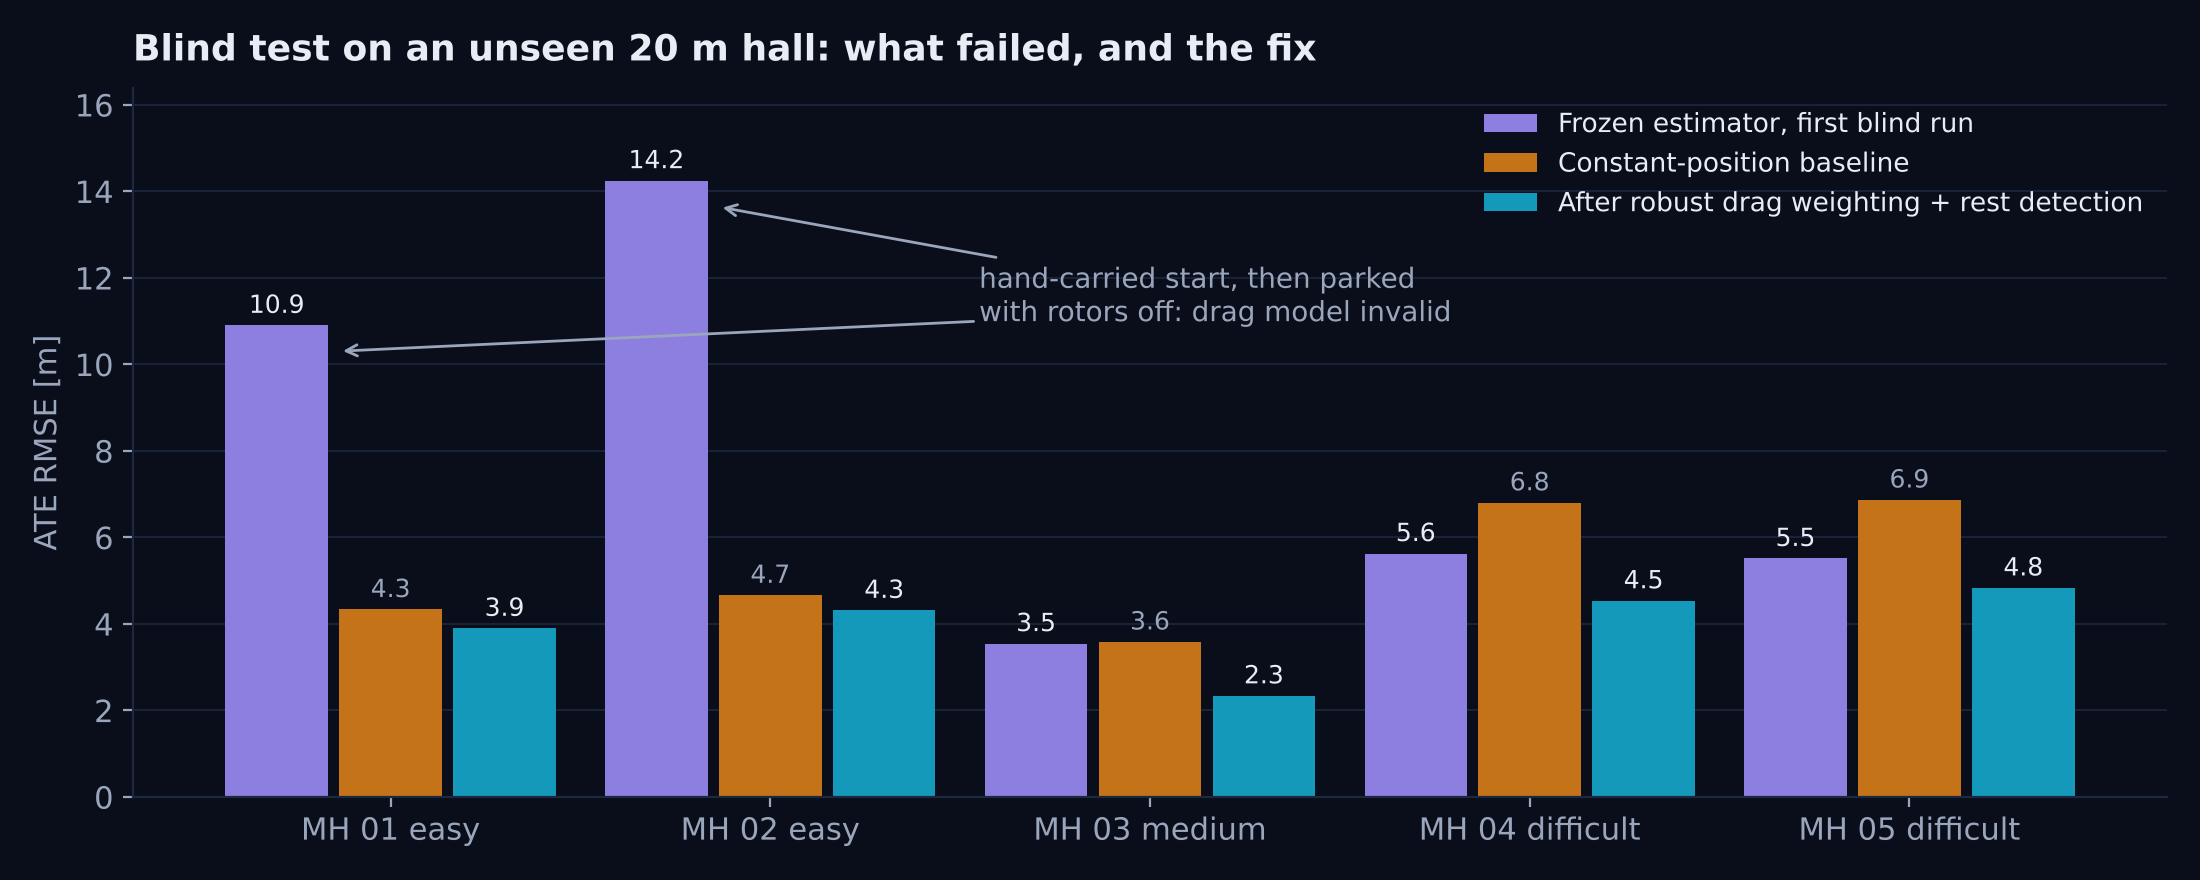
\includegraphics[width=\columnwidth]{../docs/figures/mh_blind.png}\caption{Machine Hall blind run: frozen estimator, constant reference, and after the fix.}\label{fig:mh}\end{figure}
\begin{figure}[!htb]\centering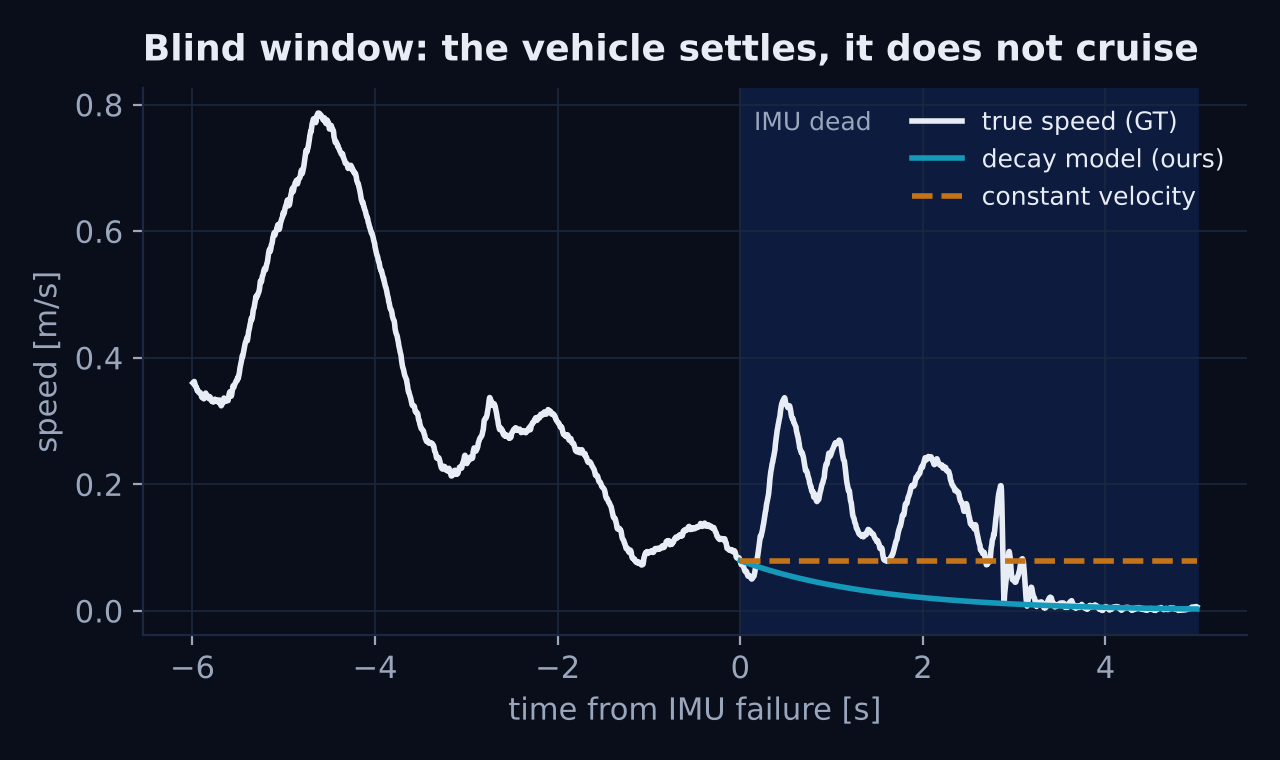
\includegraphics[width=\columnwidth]{../docs/figures/blind.png}\caption{Blind-window error against the post-failure velocity decay $\tau$, over 34 files. The same setting was selected in all 17 leave-one-sequence-out folds.}\label{fig:blind}\end{figure}

\section{How much to trust the numbers}
\begin{itemize}
\item \textbf{Nested cross-validation.} Re-choosing the workspace prior and the robust threshold on the other sequences only gives an ATE within 0.3\% and 0.7\% of the shipped numbers. Every held-out file still beats the reference (worst ratio 0.92).
\item \textbf{Other degradation draws.} Seeds 1, 7 and 2026, a milder ramp, an earlier ramp and 100\,Hz input, on six sequences including the hardest: 36/36 beat the reference.
\item \textbf{Other hardware.} On a Windows laptop (Ryzen 7 6800H, NumPy 1.26) the trajectory is bit-identical; 3.0\,MB heap and 2.4\,ms per second of data (budgets: 8\,MB, 20\,ms).
\item \textbf{Input contract.} 15 format variants (zip, folder, accelerometer-first columns, units, unsorted rows, \dots) all pass with identical ATE.
\end{itemize}

\section{Limitations}
An IMU alone cannot observe slow position. In the blind window on handheld TUM-VI motion we remain slightly worse than standing still (0.73 vs 0.64\,m), and margins on MH\_01/02 are about 8--10\%. The workspace prior assumes indoor operation. The workspace prior, the robust threshold and the blind decay were chosen with all sequences in view; the nested cross-validation bounds the resulting optimism at under 1\%.

\small
\section*{References}
\begin{enumerate}[label={[\arabic*]}]
\item M. Burri et al., The EuRoC micro aerial vehicle datasets, IJRR, 2016.
\item D. Schubert et al., The TUM VI benchmark for evaluating visual-inertial odometry, IROS, 2018.
\item R. Leishman et al., Quadrotors and accelerometers: state estimation with an improved dynamic model, IEEE CSM, 2014.
\item H. Rauch, F. Tung, C. Striebel, Maximum likelihood estimates of linear dynamic systems, AIAA J., 1965.
\item R. Mahony, T. Hamel, J.-M. Pflimlin, Nonlinear complementary filters on the special orthogonal group, IEEE TAC, 2008.
\item M. Grupp, evo: Python package for the evaluation of odometry and SLAM, 2017.
\end{enumerate}
\end{document}
